% %
% LAYOUT_E.TEX - Short description of REFMAN.CLS
%                                       99-03-20
%
%  Updated for REFMAN.CLS (LaTeX2e)
%
\documentclass[twoside,a4paper]{refart}
\usepackage{makeidx}
\usepackage{ifthen}
\usepackage[ampersand]{easylist}
\usepackage[pdftex]{graphicx}
\usepackage{float}
\usepackage{paralist}
\usepackage[doublespacing]{setspace}

% ifthen wird vom Bild von N.Beebe gebraucht!

\def\bs{\char'134 } % backslash in \tt font.
\newcommand{\ie}{i.\,e.,}
\newcommand{\eg}{e.\,g..}
\DeclareRobustCommand\cs[1]{\texttt{\char`\\#1}}

\title{Echo Cancellation Core (4-lag) Based on LSM Algorithm}
\author{
Ankai Liu \\
2018-09-06
}

\date{}
\emergencystretch1em  %

\pagestyle{myfootings}
\markboth{Echo Cancellation Core (4-lag) Based on LSM Algorithm }%
         {Echo Cancellation Core (4-lag) Based on LSM Algorithm }

\makeindex 

\setcounter{tocdepth}{2}

\begin{document}
	
\graphicspath{ {image/} }
\maketitle
\begin{abstract}
	This document is a user manual for echo cancellation core (4-lag) based on LSM algorithm. 
\end{abstract}
%\begin{spacing}{0.005}
%\tableofcontents
%\end{spacing}
%\newpage


%%%%%%%%%%%%%%%%%%%%%%%%%%%%%%%%%%%%%%%%%%%%%%%%%%%%%%%%%%%%%%%%%%%%
\section{Introduction}
This document is a user manual for echo cancellation core (4-lag) based on LSM algorithm. The core is designed on CYCLONE IV FPGAs. It is serving for a SPECIFIC signal type (16 bit binary signal with the first digit represent the sign) and a specific echo type (echo caused by transmission within the circuit).

In the project, we have implemented 4-lag and 16-lag cores that takes continuous sampling. The whole core only require gate-logic calculations. We will provide 3 test bench in order to cover all submodules for potential future modifications. 

%%%%%%%%%%%%%%%%%%%%%%%%%%%%%%%%%%%%%%%%%%%%%%%%%%%%%%%%%%%%%%%%%%%%%
\section{echo\_cancelation\_full}
Top level module. 
\begin{figure}[H]
	\centering
	\includegraphics[scale=0.7]{echo_cancelation_full.png}
	\caption{echo\_cancelation\_full hierarchy}
	\label{}
\end{figure}
\begin{figure}[H]
	\centering
	\includegraphics[scale=1.2]{echo_cancelation_full_module.png}
	\caption{echo\_cancelation\_full}
	\label{}
\end{figure}
\subsection{Input}
\begin{itemize}
		\item[clk\_operation:] Global operation clocks.
		\item[sampling\_cycle\_counter:] Global sampling clocks.
		\item[rst:      ] Global reset.
		\item[enable:] Local input. Needs to stay 1 when using the module.
		\item[set\_max\_iteration:] Local input. Set to be the numbers of iterations that users wants to achieve.
		\item[sig16b:] Original signal from sender in 16 bits binary formate.
		\item[sig16b\_lag:] Signal with lag fro receiver in 16 bits binary formate.
\end{itemize}
\subsection{Output}
\begin{itemize}
	\item[para\_approx:] Approximate parameters.
	\item[iteration:] Numbers of iterations that has been done.
	\item[sig16b\_without\_echo:] Approximation of original signal/signal without the echo in 16 bits binary formate.
\end{itemize}
\subsection{Important}
\begin{itemize}
	\item The echo\_cancelation\_full core takes new sample when "sampling\_cycle\_counter = 0". The reset cycle of sampling\_cycle\_counter must be more than 1200 of the operation clks/600 of operation cycles.
	\item The recommenced maximum iteration is 64 for lag 4. See LSM\_algorithm\_demo.pdf for details.
\end{itemize}
%%%%%%%%%%%%%%%%%%%%%%%%%%%%%%%
\section{sig16b\_to\_double}
Transforming 16 bit binary signal to double.
\begin{figure}[H]
	\centering
	\includegraphics[scale=1.2]{sig16b_to_double.png}
	\caption{sig16b\_to\_double}
	\label{}
\end{figure}
\subsection{Input}
\begin{itemize}
	\item[clk\_operation:] Global operation clocks.
	\item[rst:   ] Global reset.
	\item[enable:] Local input. Turn on for 2 operation cycles/4 operation clks and then turn off.
	\item[sig16b:] Input signal in 16 bit binary formate.
\end{itemize}
\subsection{output}
\begin{itemize}
	\item[double:] Output signal in double.
	\item[ready:] 1 for ready.
\end{itemize}
%%%%%%%%%%%%%%%%%%%%%%%%%%%%%%%%%%
\section{double\_to\_sig16b}
Transform data types from double to 16 bit binary signal
\begin{figure}[H]
	\centering
	\includegraphics[scale=1.2]{double_to_sig16b.png}
	\caption{double\_to\_sig16b}
	\label{}
\end{figure}
\subsection{Input}
\begin{itemize}
	\item[sampling\_cycle\_counter:] Global sampling clocks.
	\item[clk\_operation:] Global operation clocks.
	\item[rst:      ] Global reset.
	\item[enable:] Local input. Needs to stay 1 when using the module.
	\item[double:] Input in double.
\end{itemize}
\subsection{Output}
\begin{itemize}
	\item[sig16b:] Output in 16 bit binary formate.
\end{itemize}
%%%%%%%%%%%%%%%%%%%%%%%%%%%%%%%%%%
\section{para\_approx}
Estimate parameters for given original signals and signals with lags.
\begin{figure}[H]
	\centering
	\includegraphics[scale=1.2]{para_approx.png}
	\caption{para\_approx}
	\label{}
\end{figure}
\subsection{Input}
\begin{itemize}
		\item[rst:      ] Global reset.
		\item[sampling\_cycle\_counter:] Global sampling clocks.
		\item[clk\_operation:] Global operation clocks.
		\item[enable\_sampling:] Local input. In order to make sure the samplings are aligned, needs to stay on even the module is not operating.
		\item[enable:] Local input. Turn on for 2 operation cycles/4 operation clks and then turn off.
		\item[signal:] Input signal in double.
		\item[signal\_lag:] Input lag signal in double
		\item[gamma:] Default is\\ 64'b0011111111010000000000000000000000000000000000000000000000000000(0.01)
		\item[mu:   ] Default is\\ 64'b0011111111110000000000000000000000000000000000000000000000000000(1)
		
\end{itemize}
\subsection{Output}
\begin{itemize}
	\item[parameters:] Estimate parameters in double.
	\item[e:] Unbiased error of prediction
	\item[e\_exp:] Exponential of unbiased error of prediction
	\item[normalize\_amp\_exp:] Exponential of amplitude of normalization. For debug purpose.
	\item[ready:] 1 for ready
\end{itemize}

%%%%%%%%%%%%%%%%%%%%%%%%%%%%%%%%%%
\section{echo\_cancelation}
Preform echo cancellation for given parameters, original signals and signal with lags. 
\begin{figure}[H]
	\centering
	\includegraphics[scale=1.2]{echo_cancelation.png}
	\caption{echo\_cancelation}
	\label{}
\end{figure}
\subsection{Input}
\begin{itemize}
	\item[rst:      ] Global reset.
	\item[sampling\_cycle\_counter:] Global sampling clocks.
	\item[clk\_operation:] Global operation clocks.
	\item[enable\_sampling] Local input. In order to make sure the samplings are aligned, needs to stay on even the module is not operating.
	\item[enable:] Local input. Turn on for 2 operation cycles/4 operation clks and then turn off.
	\item[signal\_reveive:] Signals with echo in double.
	\item[signal\_send:] Original signals in double.
	\item[parameters:] Estimate parameters
\end{itemize}
\subsection{Output}
\begin{itemize}
	\item[signal\_without\_echo:] Signal after echo cancellation in double
	\item[signal\_without\_echo\_exp:] Exponential of output signal. For debug purpose.
	\item[ready:] 1 for ready.
\end{itemize}
%%%%%%%%%%%%%%%%%%%%%%%%%%%%%%%%%%
\section{lag\_generator}
Generate lag signal for given original signal and parameters.
\begin{figure}[H]
	\centering
	\includegraphics[scale=1.2]{lag_generator.png}
	\caption{lag\_generator}
	\label{}
\end{figure}
\subsection{Input}
\begin{itemize}
	\item[rst:      ] Global reset.
	\item[enable\_sampling] Local input. In order to make sure the samplings are aligned, needs to stay on even the module is not operating.
	\item[enable:] Local input. Turn on for 2 operation cycles/4 operation clks and then turn off.
	\item[sampling\_cycle\_counter:] Global sampling clocks.
	\item[clk\_operation:] Global operation clocks.
	\item[signal:] Signals with echo in double.
	\item[parameters:] Estimate parameters
\end{itemize}
\subsection{Output}
\begin{itemize}
	\item[signal\_lag:] Signal after echo cancellation in double
	\item[signal\_align:] Exponential of output signal. For debug purpose.
	\item[ready:] 1 for ready.
\end{itemize}
%%%%%%%%%%%%%%%%%%%%%%%%%%%%%%%%%%
\section{double\_16b\_tb}
Test bench for data conversion modules:\\
double\_to\_sig16b.v\\
sig16b\_to\_double.v\\
\begin{figure}[H]
	\centering
	\includegraphics[scale=1]{double_16b_tb.png}
	\caption{double\_16b\_tb hierarchy}
	\label{}
\end{figure}
%%%%%%%%%%%%%%%%%%%%%%%%%%%%%%%%%%
\section{tb\_all}
Test bench for all sub-level modules:\\
sig16b\_to\_double.v\\
lag\_generator.v\\
para\_approx.v\\
echo\_cancelation.v\\
double\_to\_sig16b.v\\
\begin{figure}[H]
	\centering
	\includegraphics[scale=0.6]{tb_all.png}
	\caption{tb\_all hierarchy}
	\label{}
\end{figure}
%%%%%%%%%%%%%%%%%%%%%%%%%%%%%%%%%%
\section{echo\_cancelation\_full\_tb}
Test bench for top-level module:\\
echo\_cancelation\_full.v\\
\begin{figure}[H]
	\centering
	\includegraphics[scale=0.7]{echo_cancelation_full_tb.png}
	\caption{echo\_cancelation\_full\_tb hierarchy}
	\label{}
\end{figure}
%%%%%%%%%%%%%%%%%%%%%%%%%%%%%%%%%%%%%%%%%%%%%%%%%%%%%%%%%%%%%%%%%%%%%%


%%%%%%%%%%%%%%%%%%%%%%%%%%%%%%%%%%%%%%%%%%%%%%%%%%%%%%%%%%%%%%%%%%%%%%

\printindex
\end{document}
